\item \textbf{Corn.  [12 pts]} Yield of corn (bushels per acre) in Nebraska counties in 2009 can be described by a Normal distribution with a mean of 178 bushels per acre and a standard deviation of 16 bushels per acre. Use \textbf{the 68-95-99.7 Rule (Empirical Rule)} to answer the following questions. (Hint: Draw pictures of the normal curve.) 
\begin{enumerate}
\item \textbf{[4 pts]} The middle $68\%$ of counties have a corn yield \textbf{between} what two values? \\
\begin{center}
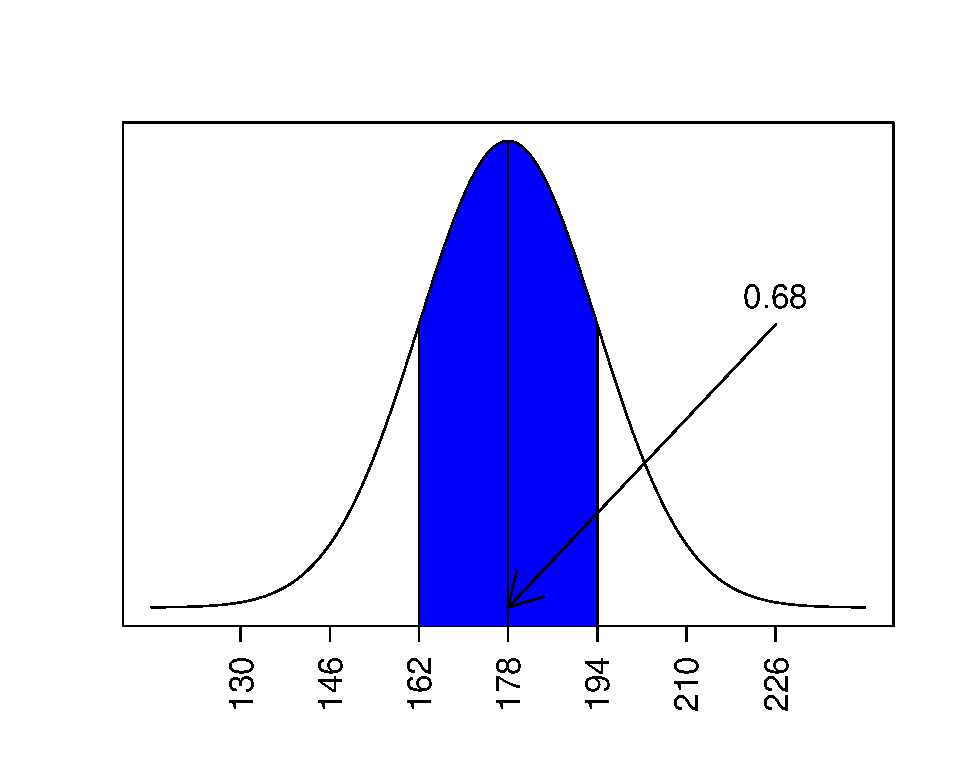
\includegraphics[scale=0.5]{corn/2a.pdf}
\end{center}
\red{$(\mu-\sigma, \mu+\sigma)$ = (178 - 16, 178 + 16) = 162 to 194 bushels per acre}

\newpage

\item \textbf{[2 pts]} What is the value of the $84^{th}$ percentile of corn yield for counties in Iowa?\\
\begin{center}
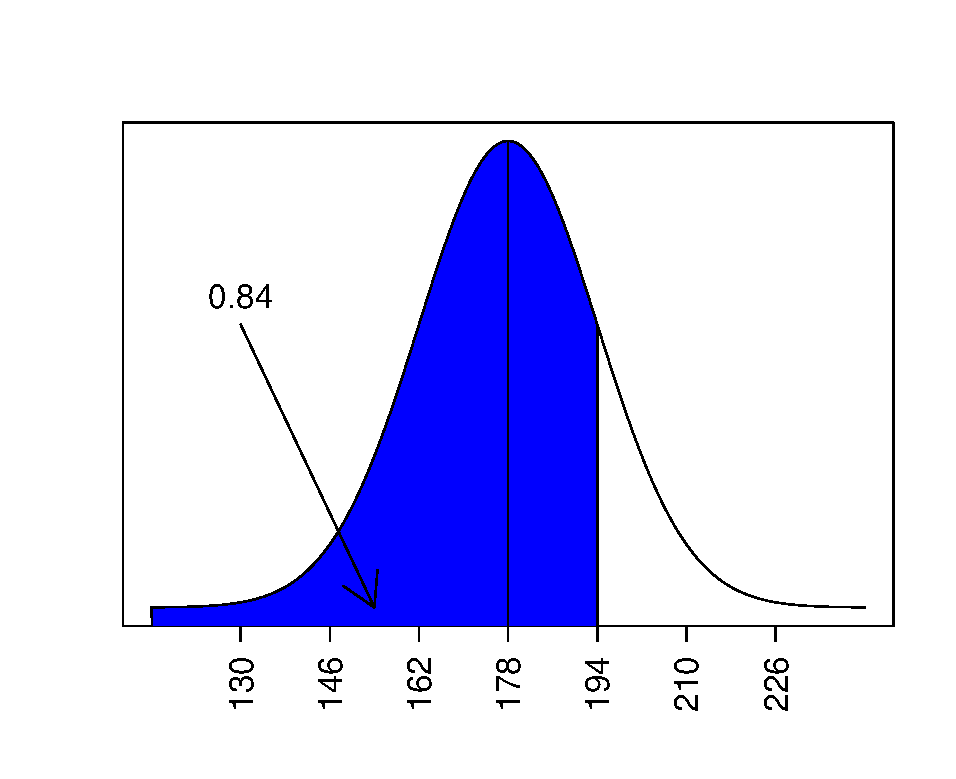
\includegraphics[scale=0.5]{corn/2b.pdf}
\end{center}
\red{In the previous part, we found that the middle 68\% of counties have a corn yield between 162 and 194 bushels per acre. This implies that $\frac{100-68}{2}=16$\% of counties have a corn yield greater than 194 bushels per acre which also implies 84\% of counties have a corn yield less than 194 bushels per acre.  So 194 bushels per acre is the value of the $84^{th}$ percentile.}

\item \textbf{[2 pts]} What proportion of counties have a corn yield \textbf{between} 162 and 226 bushels per acre?\\
\begin{center}
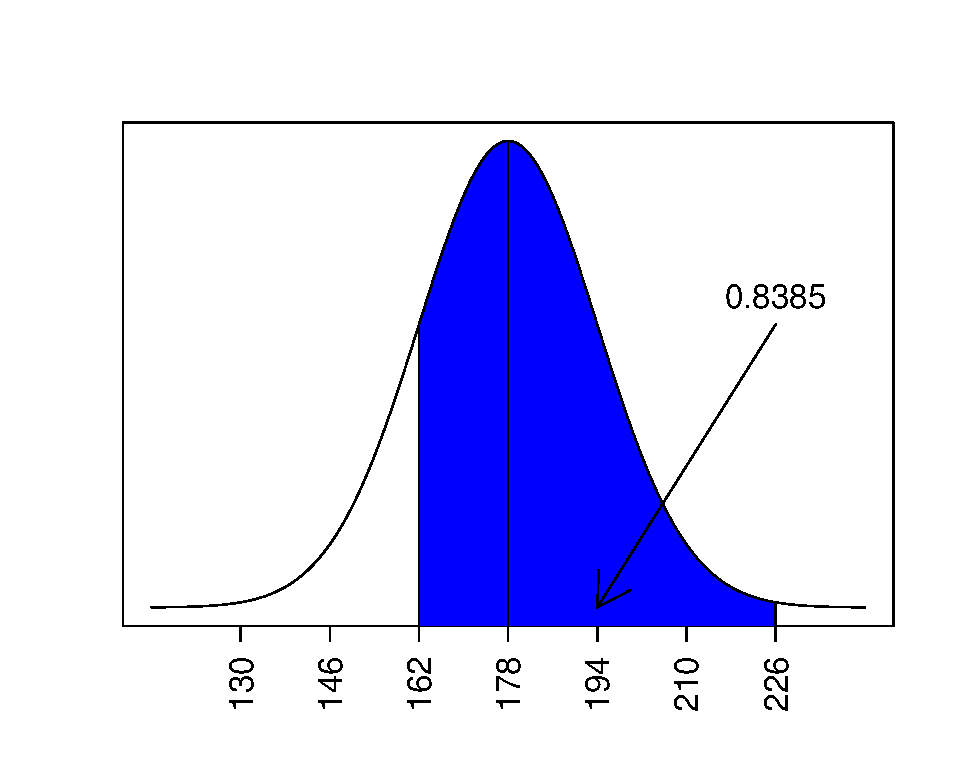
\includegraphics[scale=0.5]{corn/2c.pdf}
\end{center}
\red{Previously, we found that the middle 68\% of counties have a corn yield between 162 and 194 bushels per acre.  This implies that $\frac{68}{2}=34$\% of counties have corn yields between 162 and 178 bushels per acre.  99.7\% of counties have corn yields between $(\mu-3\sigma$, $\mu+3\sigma) = (178-48, 178+48) = (130, 226)$.  This implies that $\frac{99.7}{2}=49.85$\% of counties have corn yields between 178 and 226 bushels per acre.  Therefore, $34+ 49.85 = 83.85$\% of counties have corn yields between 162 and 226 bushels per acre.  So, the proportion of counties with corn yields between 162 and 226 bushels per acre is 0.8385.}

\newpage

\item \textbf{[2 pts]} $0.15\%$ of counties have a corn yield \textbf{less than} or equal to what value?\\
\begin{center}
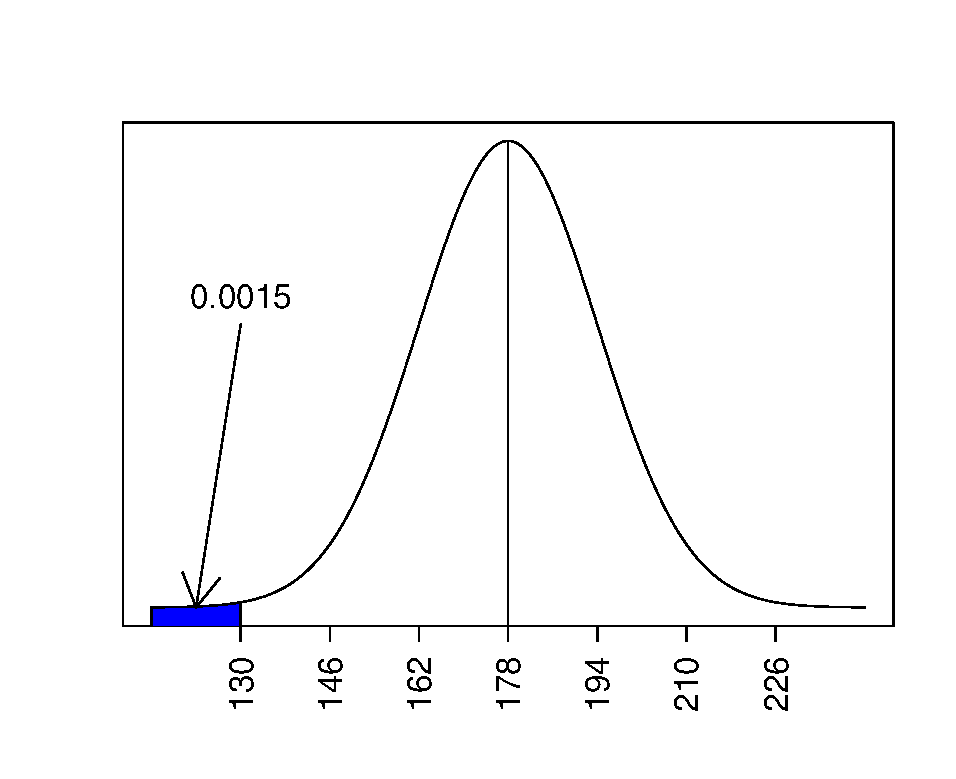
\includegraphics[scale=0.5]{corn/2d.pdf}
\end{center}
\red{99.7\% of counties have corn yields between $(\mu-3\sigma$, $\mu+3\sigma) = (178-48, 178+48) = (130, 226)$.  This implies the middle 99.7\% of counties have corn yields between 130 and 226 bushels per acre. Therefore, 0.15\% of counties have a corn yield less than 130 bushels per acre.}

\item  \textbf{[2 pts]} What proportion of counties have a corn yield of \textbf{at least} 210 bushels per acre?\\
\begin{center}
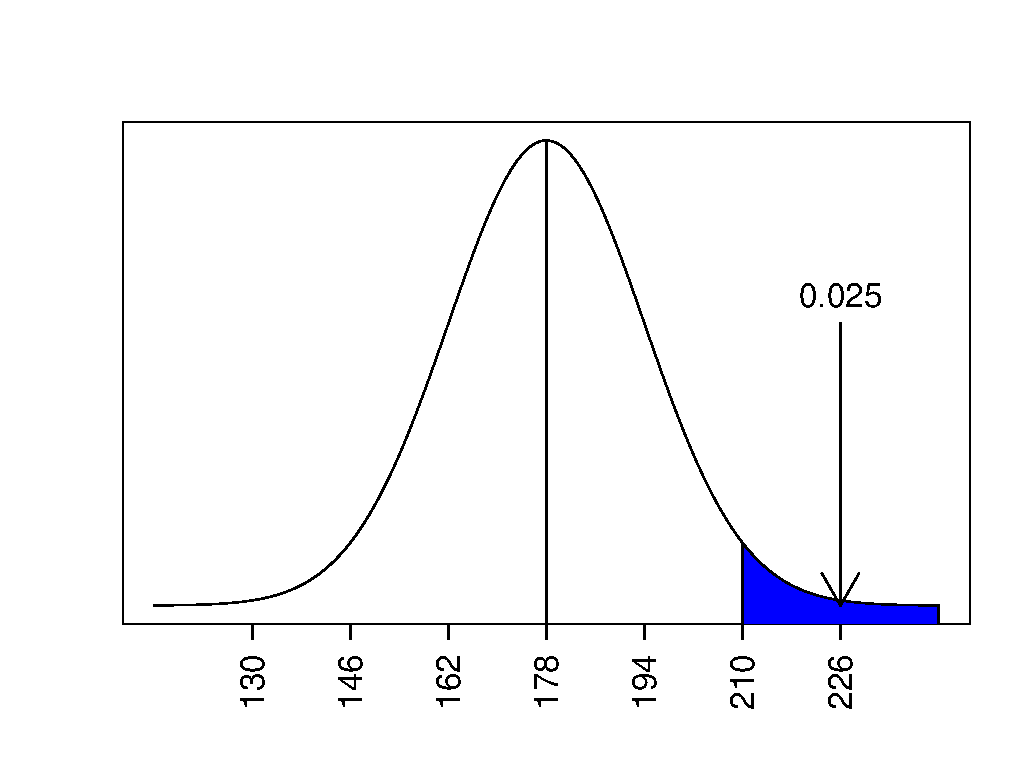
\includegraphics[scale=0.5]{corn/2e.pdf}
\end{center}
\red{95\% of counties have corn yields between $(\mu-2\sigma$, $\mu+2\sigma) = (178-32, 178+32) = (146, 210)$.  This implies the middle 95\% of counties have corn yields between 146 and 210 bushels per acre. Therefore, 2.5\% of counties have a corn yield greater than 210 bushels per acre. So, the proportion of counties with a corn yield of at least 210 bushels per acre is 0.0250.}
\end{enumerate}
